



\chapter{Fonction carrée, fonction cube}



\section{La fonction carrée}
\subsection{Définition}
  \begin{minipage}[c]{0.6\linewidth}
\begin{Définition}
La fonction carrée est la fonction définie sur $\R$ par $f:x\mapsto x^2$.
\end{Définition}
  \end{minipage} \hfill
  \begin{minipage}[c]{0.33\linewidth}
  \begin{Exemple}
  \leavevmode\vspace{-\baselineskip}
\begin{itemize}[label=\textcolor{Couleur8}{$\bullet$}]
\item $f(3)=$ \ligne 
\item $f(-8)=$ \ligne 
\end{itemize}
\end{Exemple}
  \end{minipage}


\subsection{Représentation graphique}
\begin{center}

\begin{tabular}{|c|c|c|c|c|c|c|c|c|c|}
\arrayrulecolor{Couleur6} \hline
$x$ & $-4$ & $-3$ & $-2$ & $-1$ & $0$ & $1$ & $2$ & $3$ & $4$\\
\hline
$f(x)=x^2$ & $16$ & $9$ & $4$ & $1$ & $0$ & $1$ & $4$ & $9$ & $16$\\
\hline

\end{tabular}
\end{center}

  \begin{minipage}[c]{0.4\linewidth}
  \begin{center}

\begin{tikzpicture}[scale=0.9]
\begin{axis}[
    width=10cm,
    height=10cm,
    axis lines=middle,
    grid=both,
    grid style={line width=.1pt, draw=gray!30},
    major grid style={line width=.2pt,draw=gray!30},
    xmin=-5.5, xmax=5.5,
    ymin=-0.5, ymax=11.5,
    xlabel={$x$},
    ylabel={$y$},
    xlabel style={at={(axis description cs:1.02,0.02)}, anchor=west},
    ylabel style={at={(axis description cs:0.5,1.02)}, anchor=south},
    xtick={-5,-4,-3,-2,-1,0,1,2,3,4,5},
    ytick={0,1,2,3,4,5,6,7,8,9,10,11},
    tick label style={font=\small},
    axis line style={-stealth},
]

% Tracé de la parabole y = x²
\addplot[
    domain=-3.5:3.5,
    samples=100,
    color=Couleur6,
    thick,
] {x^2};

% Étiquette de la fonction
\node at (-4.5,10.5) {$y = x^2$};

\end{axis}
\end{tikzpicture}

\end{center}
  \end{minipage} \hfill
  \begin{minipage}[c]{0.55\linewidth}
  \begin{Définition}
  La représentation graphique de la fonction carrée s'appelle un {\bf{parabole}}. Le point $O(0;0)$, origine du repère, est appelé le sommet de la parabole.
  
  \end{Définition}
  
  \begin{Propriété*}
${\color{Couleur2}{\bullet}}$ La courbe représentative de la fonction carrée admet l'axe des ordonnées pour axe de symétrie.\\
${\color{Couleur2}{\bullet}}$ Pour tout $x\in \R$, $(-x)^2=x^2$ donc $f(-x)=f(x)$, on dit que la fonction carrée est paire.
  \end{Propriété*}
  \end{minipage}
\subsection{Variations de la fonction carrée}
 \begin{minipage}[c]{0.45\linewidth}
\begin{Propriété}
La fonction carrée est décroissante sur $]-\infty;0]$ et croissante sur $[0;+\infty[$.
\end{Propriété}
On peut dresser le tableau de variations.
\begin{center}
  \begin{tikzpicture}
      \tkzTabInit[espcl=2,lgt=3]{$x$ / 1, Variations de $f(x)=x^2$ /2 } { $-\infty$ , $0$ , $+\infty$ };
\tkzTabVar{ +/ ,  -/$0$, +/ };
      \end{tikzpicture} 
      \end{center}
  \end{minipage} \hfill
  \begin{minipage}[c]{0.5\linewidth}
  \begin{proof}~\\
  Montrons que $f$ est croissante sur $\intfo{0}{+\infty}$.\\
  Pour cela, prenons $a$ et $b$ deux réels de l'intervalle $\intfo{0}{+\infty}$ tels que $a\leq b$. \\Montrons alors que $f(a)\leq f(b)$, c'est-à-dire $a^2\leq b^2$.\\
  On étudie donc le signe de $a^2-b^2$. \\
  On a $a^2-b^2=(a+b)(a-b)$. \\
  Comme $a\leq b$, $(a-b)\leq 0$ ; \\et comme $a$ et $b$ sont positifs, $(a+b)$ est positif.\\
  On en déduit que le produit $\underbrace{(a+b)}_{\color{Couleur8}{\geq 0}}\underbrace{(a-b)}_{\color{Couleur8}{\leq 0}}\leq 0$.\\ Donc $a^2-b^2\leq 0$, d'où $f(a)-f(b)\leq 0$ et donc \\$f(a)\leq f(b)$, ce qu'on souhaitait. \\
  Ainsi, $f$ est croissante sur $[0;+\infty[$.\\
  On conclut par symétrie de la courbe de $f$ par rapport à l'axe des ordonnées, que $f$ est décroissante sur $]-\infty;0]$.
  \end{proof}
  \end{minipage}

\newpage


\section{La fonction cube}
\subsection{Définition}
  \begin{minipage}[c]{0.6\linewidth}
\begin{Définition}
La fonction cube est la fonction définie sur $\R$ par $f:x\mapsto x^3$.
\end{Définition}
  \end{minipage} \hfill
  \begin{minipage}[c]{0.33\linewidth}
  \begin{Exemple}
  \leavevmode\vspace{-\baselineskip}
\begin{itemize}[label=\textcolor{Couleur8}{$\bullet$}]
\item $f(3)=$ \ligne 
\item $f(-1)=$ \ligne 
\end{itemize}
\end{Exemple}
  \end{minipage}


\subsection{Représentation graphique}
\begin{center}

\begin{tabular}{|c|c|c|c|c|c|c|c|c|c|}
\arrayrulecolor{Couleur6} \hline
$x$ & $-4$ & $-3$ & $-2$ & $-1$ & $0$ & $1$ & $2$ & $3$ & $4$\\
\hline
$f(x)=x^3$ & $-64$ & $-27$ & $-8$ & $-1$ & $0$ & $1$ & $8$ & $27$ & $64$\\
\hline

\end{tabular}
\end{center}

  \begin{minipage}[c]{0.4\linewidth}
  \begin{center}
\begin{tikzpicture}[scale=0.9]
\begin{axis}[
    width=10cm,
    height=12cm,
    axis lines=middle,
    grid=both,
    grid style={line width=.1pt, draw=gray!30},
    major grid style={line width=.2pt,draw=gray!30},
    xmin=-6.5, xmax=6.5,
    ymin=-10.5, ymax=10.5,
    xlabel={$x$},
    ylabel={$y$},
    xlabel style={at={(axis description cs:1,0.5)}, anchor=west},
    ylabel style={at={(axis description cs:0.5,1.02)}, anchor=south},
    xtick={-6,-5,-4,-3,-2,-1,0,1,2,3,4,5,6},
    ytick={-10,-9,-8,-7,-6,-5,-4,-3,-2,-1,0,1,2,3,4,5,6,7,8,9,10},
    tick label style={font=\small},
    axis line style={-stealth},
]

% Tracé de la fonction exponentielle y = x³
\addplot[
    domain=-2.2:2.2,
    samples=200,
    color=Couleur6,
    thick,
] {x^3};

% Étiquette de la fonction
\node[anchor=south west] at (axis cs:2.5,8) {$y = x^3$};

\end{axis}
\end{tikzpicture}
\end{center}
  \end{minipage} \hfill
  \begin{minipage}[c]{0.55\linewidth}

  
  \begin{Propriété*}
${\color{Couleur2}{\bullet}}$ La courbe représentative de la fonction cube admet \\l'origine $O(0;0)$ comme centre de symétrie.\\
${\color{Couleur2}{\bullet}}$ Pour tout $x\in \R$, $(-x)^3=-x^3$ donc $f(-x)=-f(x)$, on dit que la fonction cube est impaire.
  \end{Propriété*}
  \end{minipage}
  
  \vspace{0.5cm}
  
\subsection{Variations de la fonction cube}
\begin{Propriété}
La fonction cube est croissante sur $\R$.
\end{Propriété}
On peut dresser le tableau de variations.
\begin{center}
  \begin{tikzpicture}
      \tkzTabInit[espcl=5,lgt=3]{$x$ / 1, Variations de $f(x)=x^3$ /2 } { $-\infty$  , $+\infty$ };
\tkzTabVar{ -/ ,  +/ };
      \end{tikzpicture} 
      \end{center}

\newpage

\section{Équations et inéquations}
\begin{minipage}[c]{0.75\linewidth}
\subsection{Résolution d'équations}

\begin{Propriété}
Pour tout réel $a$, l'équation $x^2=a$ admet :
\begin{itemize}[label=\textcolor{Couleur2}{$\bullet$}]
\item deux solutions $\sqrt{a}$ et $-\sqrt{a}$ si $\color{Couleur6}{a>0}$ ; 
\item une unique solution égale à $0$ si $\color{Couleur8}{a=0}$ ; 
\item aucune solution si $\color{Couleur3}{a<0}$ ; 
\end{itemize}
\end{Propriété}
\end{minipage} \hfill
\begin{minipage}[c]{0.25\linewidth}
\begin{tikzpicture}[x=0.8cm,y=0.8cm]


% Axes
\draw[thick,->] (-2.5,0) -- (2.5,0);
\draw[thick,->] (0,-1.2) -- (0,3.5);

% Labels des axes (exactement comme dans votre code)
\draw (0,0) node[below left] {0};
\draw (2.2,0) node[below ] {$x$};
\draw (0,3.2) node[left] {$y$};

% Fonction y = x² (exactement comme dans votre code)
\draw[samples=300,domain=-1.8:1.8,thick] plot(\x,\x*\x) ;


% Segments horizontaux (exactement comme dans votre code)
\draw[Couleur8,very thick] (-2.5,0)--(2.5,0);
\draw[Couleur3, very thick] (-2.5,-1)--(2.5,-1);

% Labels pour a<0 et a>0 (avec des couleurs standard)
\draw[Couleur6] (0,-1) node[above,Couleur3] {$a<0$};
\draw[Couleur6, very thick] (-2.5,2.2)--(2.5,2.2);
\draw[Couleur6] (0,2.2) node[below,Couleur6] {$a>0$};

% Lignes pointillées verticales (exactement comme dans votre code)
\draw[dotted,thick] (-1.48324,0) node[below,Couleur6]{$-\sqrt{a}$}--(-1.48324,2.2);
\draw[dotted,thick] (1.48324,0) node[below,Couleur6]{$\sqrt{a}$}--(1.48324,2.2);

% Graduations (exactement comme dans votre code)
\foreach \x in {1}\draw(\x, 1pt)--(\x,-1pt) node[below] {$\x$}; 
\foreach \y in {1}\draw(1pt,\y)--(-1pt,\y) node[left] {$\y$};

\end{tikzpicture}
\end{minipage}


\begin{Propriété}
Pour tout réel $a$, l'équation $x^3=a$ admet une unique solution, appelée racine cubique de $a$, et notée $\sqrt[3]{a}$.
\end{Propriété}
\vspace{0.2cm}
\begin{minipage}[c]{0.7\linewidth}
\subsection{Résolutions d'inéquations}
\begin{Propriété}
Pour tout réel $a$, l'inéquation $\color{Couleur8}{x^2\leq a}$ admet pour ensemble de solutions :
\begin{itemize}[label=\textcolor{Couleur2}{$\bullet$}]
\item $S=\intff{-\sqrt{a}}{\sqrt{a}}$ si $\color{Couleur6}{a>0}$ ; 
\item $S=\{0\}$ si $\color{Couleur8}{a=0}$ ; 
\item $S=\emptyset$ si $\color{Couleur3}{a<0}$ ; 
\end{itemize}
Pour tout réel $a$, l'inéquation $\color{pink}{x^2\geq a}$ admet pour ensemble de solutions :
\begin{itemize}[label=\textcolor{Couleur2}{$\bullet$}]
\item $S=\intof{-\infty}{-\sqrt{a}}\cup\intfo{\sqrt{a}}{+\infty}$ si $\color{Couleur8}{a>0}$ ; 
\item $S=\R$ si $\color{Couleur3}{a\leq 0}$ ; 
\end{itemize}
\end{Propriété}
\end{minipage} \hfill
\vspace{0.3cm}
\begin{minipage}[c]{0.25\linewidth}
\begin{tikzpicture}[x=0.8cm,y=0.8cm]

% Axes
\draw[thick,->] (-2.5,0) -- (2.5,0);
\draw[thick,->] (0,-1.2) -- (0,3.5);

% Labels des axes
\draw (0,0) node[below left] {0};
\draw (2.2,0) node[below ] {$x$};
\draw (0,3.2) node[left] {$y$};

% Fonction y = x² en trois parties avec couleurs différentes
\draw[samples=300,domain=-1.48324:1.48324,thick,Couleur8] plot(\x,\x*\x) ;
\draw[samples=300,domain=-1.9:-1.48324,thick,pink] plot(\x,\x*\x) ;
\draw[samples=300,domain=1.48324:1.9,thick,pink] plot(\x,\x*\x) ;


% Segments horizontaux
\draw[Couleur3,thick] (-2.5,0)--(2.5,0);
\draw[Couleur6,thick] (-2.5,-1)--(2.5,-1);

% Labels pour a<0 et a>0
\draw[Couleur8] (0,-1) node[above,Couleur3] {$a<0$};
\draw[Couleur8,thick] (-2.5,2.2)--(2.5,2.2);
\draw[Couleur6] (0,2.2) node[below,Couleur8] {$a>0$};

% Lignes pointillées verticales
\draw[dotted,thick] (-1.48324,0) node[below,Couleur6]{$-\sqrt{a}$}--(-1.48324,2.2);
\draw[dotted,thick] (1.48324,0) node[below,Couleur6]{$\sqrt{a}$}--(1.48324,2.2);

% Graduations
\foreach \x in {1}\draw(\x, 1pt)--(\x,-1pt) node[below] {$\x$}; 
\foreach \y in {1}\draw(1pt,\y)--(-1pt,\y) node[left] {$\y$};

\end{tikzpicture}
\end{minipage}



\begin{minipage}[c]{0.70\linewidth}
\vspace{0.3cm}
\begin{Propriété}
Pour tout réel $a$, \begin{itemize}[label=\textcolor{Couleur2}{$\bullet$}]
\item l'inéquation $x^3\leq a$ admet pour ensemble de solution $S=]-\infty;\sqrt[3]{a}]$
\item l'inéquation $x^3\geq a$ admet pour ensemble de solution $S=[\sqrt[3]{a};\infty[$.
\end{itemize}

\end{Propriété}
\vspace{0.3cm}
\subsection{Position relative des courbes $y=x$, $y=x^2$ et $y=x^3$}
\vspace{0.3cm}
\begin{Propriété} $ $\\
\vspace{-0.5cm}
\begin{itemize}[label=\textcolor{Couleur2}{$\bullet$}]
\item Pour tout $x\in \intff{0}{1}$, on a $x^3\leq x^2\leq x$.
\item  Pour tout $x\in \intfo{1}{+\infty}$, on a $x\leq x^2\leq x^3$.
\end{itemize}
\end{Propriété}
\end{minipage} \hfill
\begin{minipage}[c]{0.25\linewidth}
\begin{tikzpicture}[x=1.5cm,y=1.5cm]

% Axes
\draw[thick,->] (-0.5,0) -- (2.5,0);
\draw[thick,->] (0,-0.5) -- (0,2.5);

% Labels des axes
\draw (0,0) node[below left] {0};
\draw (2.3,0) node[below ] {$x$};
\draw (0,2.3) node[left] {$y$};

% Fonctions
\draw[samples=300,domain=0:1.36,pink,thick] plot(\x,\x*\x*\x) ;
\draw[samples=300,domain=0:1.58,Couleur8,thick] plot(\x,\x*\x) ;
\draw[samples=300,domain=0:2.5,Couleur3,thick] plot(\x,\x) ;

% Labels des fonctions
\draw [color=pink,thick](1,2) node[left] {$y=x^3$};
\draw [color=Couleur8,thick](1,1) node[anchor=north west] {$y=x^2$};
\draw [color=Couleur3,thick](1.4,1.4) node[anchor=north west] {$y=x$};

% Graduations
\foreach \x in {1}\draw(\x, 1pt)--(\x,-1pt) node[below] {$\x$}; 
\foreach \y in {1}\draw(1pt,\y)--(-1pt,\y) node[left] {$\y$};

% Lignes pointillées
\draw[dotted] (0,1)--(1,1)--(1,0);

\end{tikzpicture}
\end{minipage}

\begin{proof}
~\\
~\\
\begin{minipage}[c]{0.5\linewidth}
 \underline{Premier cas : $0\leq x \leq 1$.}\\ 
Pour étudier les positions relatives des courbes d'équations $y=x$ et $y=x^2$, il suffit d'étudier le signe de $x^2-x$.\\
Or, $x^2-x=x(x-1)\leq 0$ car $x\geq 0$ et $x-1\leq 0$.
\\Donc, la courbe d'équation $y=x^2$ se trouve en dessous de la courbe d'équation $y=x$.\\
Pour étudier les positions relatives des courbes d'équations $y=x^2$ et $y=x^3$, il suffit d'étudier le signe de $x^3-x^2$.\\
Et, $x^3-x^2=x^2(x-1)\leq 0$ car $x^2\geq 0$ et $x-1\leq 0$. \\
Donc la courbe d'équation $y=x^3$ se trouve en dessous de la courbe d'équation $y=x^2$.

\end{minipage} \hfill
\begin{minipage}[c]{0.4\linewidth}
 \underline{Deuxième cas : $1\leq x <+\infty$.}\\
Dans ce cas, $x^2-x=x(x-1)\geq 0$ car $x\geq 1$.
\\Donc, la courbe d'équation $y=x^2$ se trouve au dessus de la courbe d'équation $y=x$.\\
Et, $x^3-x^2=x^2(x-1)\geq 0$ car $x \geq 1$. \\
Donc la courbe d'équation $y=x^3$ se trouve au dessus de la courbe d'équation $y=x^2$.
\end{minipage}
\end{proof}

\bigskip

\newpage

\section*{Exercices - Fonction carrée, fonction cube}
\addcontentsline{toc}{section}{Exercices}
{\setlength{\columnseprule}{0pt}
\setcounter{NumEx}{1}

\subsection*{Fonction carrée}


% @see : https://coopmaths.fr/alea?uuid=b6cc0&id=2F11-1&n=8&d=10&s=true&s2=false&s3=false&s4=false&alea=InLY&cd=1&cols=2
\begin{Exercice}%1
\leavevmode\vspace{-\baselineskip}
\begin{multicols}{2}
\begin{enumerate}[itemsep=1em]
	\item \begin{minipage}[t]{\linewidth}Soit $f_1$ la fonction carré.\\
      
      Calculer l'image de $6$ par la fonction $f_1$.\end{minipage}
	\item \begin{minipage}[t]{\linewidth}Soit $g_1$ la fonction carré.\\
      
      Calculer $g_1(-3)$.\end{minipage}
	\item \begin{minipage}[t]{\linewidth}Soit $h_1$ la fonction carré.\\
      
      Calculer $h_1(-9)$.\end{minipage}
	\item \begin{minipage}[t]{\linewidth}Soit $p_1$ la fonction carré.\\
      
      Calculer l'image de $-8$ par la fonction $p_1$.\end{minipage}
	\item \begin{minipage}[t]{\linewidth}Soit $q_1$ la fonction carré.\\
      
      Calculer $q_1(-7)$.\end{minipage}
	\item \begin{minipage}[t]{\linewidth}Soit $r_1$ la fonction carré.\\
      
      Calculer l'image de $-5$ par la fonction $r_1$.\end{minipage}
	\item \begin{minipage}[t]{\linewidth}Soit $s_1$ la fonction carré.\\
      
      Calculer l'image de $-2$ par la fonction $s_1$.\end{minipage}
	\item \begin{minipage}[t]{\linewidth}Soit $t_1$ la fonction carré.\\
      
      Calculer $t_1(-10)$.\end{minipage}
\end{enumerate}
\end{multicols}
\end{Exercice}

% @see : https://coopmaths.fr/alea?uuid=9315e&id=2F11-2&n=6&d=10&s=2&s2=2&alea=jLm2&cd=1&cols=1
\begin{Exercice}%2
Comparer les nombres suivants :
\begin{multicols}{3}
\begin{enumerate}[itemsep=1.5em]
	\item \begin{minipage}[t]{\linewidth}$(-3{,}872)^2$ et $(-3{,}876)^2$.\end{minipage}
	\item \begin{minipage}[t]{\linewidth}$3{,}991^2$ et $3{,}999^2$.\end{minipage}
	\item \begin{minipage}[t]{\linewidth}$(-4{,}681)^2$ et $(-4{,}669)^2$.\end{minipage}
	\item \begin{minipage}[t]{\linewidth}$1{,}951^2$ et $1{,}945^2$.\end{minipage}
	\item \begin{minipage}[t]{\linewidth}$2{,}85^2$ et $2{,}844^2$.\end{minipage}
	\item \begin{minipage}[t]{\linewidth}$(-5{,}59)^2$ et $(-5{,}574)^2$.\end{minipage}
\end{enumerate}
\end{multicols}
\end{Exercice}

% @see : https://coopmaths.fr/alea?uuid=9315e&id=2F11-2&n=6&d=10&s=2&s2=1&alea=Hy9Y&cd=1&cols=1
\begin{Exercice}%3
\leavevmode\vspace{-\baselineskip}
\begin{multicols}{2}
\begin{enumerate}[itemsep=1.5em]
	\item \begin{minipage}[t]{\linewidth} Soit $u$ la fonction carré.\\
            Sans effectuer de calcul, comparer $u(1{,}57)$ et $u(1{,}58)$. \end{minipage}
	\item \begin{minipage}[t]{\linewidth} Soit $h$ la fonction carré.\\
            Sans effectuer de calcul, comparer $h(-0{,}771)$ et $h(-0{,}777)$. \end{minipage}
	\item \begin{minipage}[t]{\linewidth} Soit $f$ la fonction carré.\\
            Sans effectuer de calcul, comparer $f(0{,}852)$ et $f(0{,}844)$. \end{minipage}
	\item \begin{minipage}[t]{\linewidth} Soit $g$ la fonction carré.\\
            Sans effectuer de calcul, comparer $g(-4{,}651)$ et $g(-4{,}655)$. \end{minipage}
	\item \begin{minipage}[t]{\linewidth} Soit $w$ la fonction carré.\\
            Sans effectuer de calcul, comparer $w(0{,}652)$ et $w(0{,}642)$. \end{minipage}
	\item \begin{minipage}[t]{\linewidth} Soit $h$ la fonction carré.\\
            Sans effectuer de calcul, comparer $h(-3{,}781)$ et $h(-3{,}785)$. \end{minipage}
\end{enumerate}
\end{multicols}
\end{Exercice}

\newpage

\subsection*{Fonction cube}

% @see : https://coopmaths.fr/alea?uuid=b6cc0&id=2F11-1&n=8&d=10&s=false&s2=true&s3=false&s4=false&alea=ugRO&cd=1&cols=2
\begin{Exercice}%4
\leavevmode\vspace{-\baselineskip}
\begin{multicols}{2}
\begin{enumerate}[itemsep=1em]
	\item \begin{minipage}[t]{\linewidth}Soit $f_1$ la fonction cube.\\
      
      Calculer $f_1(-4)$.\end{minipage}
	\item \begin{minipage}[t]{\linewidth}Soit $g_1$ la fonction cube.\\
      
      Calculer l'image de $5$ par la fonction $g_1$.\end{minipage}
	\item \begin{minipage}[t]{\linewidth}Soit $h_1$ la fonction cube.\\
      
      Calculer l'image de $4$ par la fonction $h_1$.\end{minipage}
	\item \begin{minipage}[t]{\linewidth}Soit $p_1$ la fonction cube.\\
      
      Calculer $p_1(3)$.\end{minipage}
	\item \begin{minipage}[t]{\linewidth}Soit $q_1$ la fonction cube.\\
      
      Calculer $q_1(-5)$.\end{minipage}
	\item \begin{minipage}[t]{\linewidth}Soit $r_1$ la fonction cube.\\
      
      Calculer l'image de $-2$ par la fonction $r_1$.\end{minipage}
	\item \begin{minipage}[t]{\linewidth}Soit $s_1$ la fonction cube.\\
      
      Calculer $s_1(-1)$.\end{minipage}
	\item \begin{minipage}[t]{\linewidth}Soit $t_1$ la fonction cube.\\
      
      Calculer l'image de $2$ par la fonction $t_1$.\end{minipage}
\end{enumerate}
\end{multicols}
\end{Exercice}

% @see : https://coopmaths.fr/alea?uuid=9315e&id=2F11-2&n=6&d=10&s=5&s2=2&alea=RE9V&cd=1&cols=1
\begin{Exercice}%5
Comparer les nombres suivants :
\begin{multicols}{3}
\begin{enumerate}[itemsep=1.5em]
	\item \begin{minipage}[t]{\linewidth}$(-7{,}2)^3$ et $(-6{,}8)^3$.\end{minipage}
	\item \begin{minipage}[t]{\linewidth}$(-6{,}5)^3$ et $(-6{,}7)^3$.\end{minipage}
	\item \begin{minipage}[t]{\linewidth}$(-7{,}1)^3$ et $(-7{,}8)^3$.\end{minipage}
	\item \begin{minipage}[t]{\linewidth}$7{,}7^3$ et $8{,}5^3$.\end{minipage}
	\item \begin{minipage}[t]{\linewidth}$2{,}4^3$ et $2^3$.\end{minipage}
	\item \begin{minipage}[t]{\linewidth}$(-7{,}4)^3$ et $(-8)^3$.\end{minipage}
\end{enumerate}
\end{multicols}
\end{Exercice}

% @see : https://coopmaths.fr/alea?uuid=9315e&id=2F11-2&n=6&d=10&s=5&s2=1&alea=RprA&cd=1&cols=1
\begin{Exercice}%6
\leavevmode\vspace{-\baselineskip}
\begin{multicols}{2}
\begin{enumerate}[itemsep=1.5em]
	\item \begin{minipage}[t]{\linewidth} Soit $u$ la fonction cube.\\
            Sans effectuer de calcul, comparer $u(-7{,}4)$ et $u(-7{,}7)$. \end{minipage}
	\item \begin{minipage}[t]{\linewidth} Soit $f$ la fonction cube.\\
            Sans effectuer de calcul, comparer $f(-8{,}4)$ et $f(-9{,}3)$. \end{minipage}
	\item \begin{minipage}[t]{\linewidth} Soit $u$ la fonction cube.\\
            Sans effectuer de calcul, comparer $u(-5{,}1)$ et $u(-5{,}8)$. \end{minipage}
	\item \begin{minipage}[t]{\linewidth} Soit $g$ la fonction cube.\\
            Sans effectuer de calcul, comparer $g(-10{,}9)$ et $g(-10{,}2)$. \end{minipage}
	\item \begin{minipage}[t]{\linewidth} Soit $u$ la fonction cube.\\
            Sans effectuer de calcul, comparer $u(7{,}3)$ et $u(6{,}7)$. \end{minipage}
	\item \begin{minipage}[t]{\linewidth} Soit $h$ la fonction cube.\\
            Sans effectuer de calcul, comparer $h(6{,}6)$ et $h(7)$. \end{minipage}
\end{enumerate}
\end{multicols}
\end{Exercice}

\newpage

\subsection*{Équation et inéquation}


% @see : https://coopmaths.fr/alea?uuid=de0d1&id=2F12-1&n=6&d=10&s=1&s2=1&alea=LNxe&cd=0&cols=1
\begin{Exercice}%7
\leavevmode\vspace{-\baselineskip}

\begin{multicols}{3}
\begin{enumerate}[itemsep=1em]
	\item \begin{minipage}[t]{\linewidth}Résoudre dans $\mathbb{R}$ :\\
              \,\,\,\,\,\,\,\,\,\,\,\,\,\,\,\,\,\,\,\,\,\,\,\,\,\,\,\,\,\,\,\,\,\,\,\,\,\,\,\,\,\,\,\,\,\,\,\,\,\, $x^2=64$\\\end{minipage}
	\item \begin{minipage}[t]{\linewidth}Résoudre dans $\mathbb{R}$ :\\
              \,\,\,\,\,\,\,\,\,\,\,\,\,\,\,\,\,\,\,\,\,\,\,\,\,\,\,\,\,\,\,\,\,\,\,\,\,\,\,\,\,\,\,\,\,\,\,\,\,\, $x^2=-19$\\\end{minipage}
	\item \begin{minipage}[t]{\linewidth}Résoudre dans $\mathbb{R}$ :\\
              \,\,\,\,\,\,\,\,\,\,\,\,\,\,\,\,\,\,\,\,\,\,\,\,\,\,\,\,\,\,\,\,\,\,\,\,\,\,\,\,\,\,\,\,\,\,\,\,\,\, $x^2=100$\\\end{minipage}
	\item \begin{minipage}[t]{\linewidth}Résoudre dans $\mathbb{R}$ :\\
              \,\,\,\,\,\,\,\,\,\,\,\,\,\,\,\,\,\,\,\,\,\,\,\,\,\,\,\,\,\,\,\,\,\,\,\,\,\,\,\,\,\,\,\,\,\,\,\,\,\, $x^2=-15$\\\end{minipage}
	\item \begin{minipage}[t]{\linewidth}Résoudre dans $\mathbb{R}$ :\\
              \,\,\,\,\,\,\,\,\,\,\,\,\,\,\,\,\,\,\,\,\,\,\,\,\,\,\,\,\,\,\,\,\,\,\,\,\,\,\,\,\,\,\,\,\,\,\,\,\,\, $x^2=-7$\\\end{minipage}
	\item \begin{minipage}[t]{\linewidth}Résoudre dans $\mathbb{R}$ :\\
              \,\,\,\,\,\,\,\,\,\,\,\,\,\,\,\,\,\,\,\,\,\,\,\,\,\,\,\,\,\,\,\,\,\,\,\,\,\,\,\,\,\,\,\,\,\,\,\,\,\, $x^2=26$\\\end{minipage}
\end{enumerate}
\end{multicols}
\end{Exercice}

% @see : https://coopmaths.fr/alea?uuid=de0d1&id=2F12-1&n=6&d=10&s=1&s2=2&alea=ShAi&cd=0&cols=1
\begin{Exercice}%8
\leavevmode\vspace{-\baselineskip}

\begin{multicols}{3}
\begin{enumerate}[itemsep=1em]
	\item \begin{minipage}[t]{\linewidth}Résoudre dans $\mathbb{R}$ :\\
              \,\,\,\,\,\,\,\,\,\,\,\,\,\,\,\,\,\,\,\,\,\,\,\,\,\,\,\,\,\,\,\,\,\,\,\,\,\,\,\,\,\,\,\,\,\,\,\,\,\, $-x^2-5=-5$\\\end{minipage}
	\item \begin{minipage}[t]{\linewidth}Résoudre dans $\mathbb{R}$ :\\
              \,\,\,\,\,\,\,\,\,\,\,\,\,\,\,\,\,\,\,\,\,\,\,\,\,\,\,\,\,\,\,\,\,\,\,\,\,\,\,\,\,\,\,\,\,\,\,\,\,\, $x^2-10=111$\\\end{minipage}
	\item \begin{minipage}[t]{\linewidth}Résoudre dans $\mathbb{R}$ :\\
              \,\,\,\,\,\,\,\,\,\,\,\,\,\,\,\,\,\,\,\,\,\,\,\,\,\,\,\,\,\,\,\,\,\,\,\,\,\,\,\,\,\,\,\,\,\,\,\,\,\, $-9x^2+4=-6$\\\end{minipage}
	\item \begin{minipage}[t]{\linewidth}Résoudre dans $\mathbb{R}$ :\\
              \,\,\,\,\,\,\,\,\,\,\,\,\,\,\,\,\,\,\,\,\,\,\,\,\,\,\,\,\,\,\,\,\,\,\,\,\,\,\,\,\,\,\,\,\,\,\,\,\,\, $x^2+1=-16$\\\end{minipage}
	\item \begin{minipage}[t]{\linewidth}Résoudre dans $\mathbb{R}$ :\\
              \,\,\,\,\,\,\,\,\,\,\,\,\,\,\,\,\,\,\,\,\,\,\,\,\,\,\,\,\,\,\,\,\,\,\,\,\,\,\,\,\,\,\,\,\,\,\,\,\,\, $-x^2-4=-200$\\\end{minipage}
	\item \begin{minipage}[t]{\linewidth}Résoudre dans $\mathbb{R}$ :\\
              \,\,\,\,\,\,\,\,\,\,\,\,\,\,\,\,\,\,\,\,\,\,\,\,\,\,\,\,\,\,\,\,\,\,\,\,\,\,\,\,\,\,\,\,\,\,\,\,\,\, $-5x^2+9=-7$\\\end{minipage}
\end{enumerate}
\end{multicols}
\end{Exercice}

% @see : https://coopmaths.fr/alea?uuid=277d3&id=2F12-2&n=12&d=10&s=1&alea=wqHa&cd=1&cols=1
\begin{Exercice}%9
Résoudre graphiquement les inéquations :
\begin{multicols}{4}
\begin{enumerate}[itemsep=1.5em]
	\item \begin{minipage}[t]{\linewidth} $x^2 \leqslant 22$.\end{minipage}
	\item \begin{minipage}[t]{\linewidth} $x^2>6$.\end{minipage}
	\item \begin{minipage}[t]{\linewidth} $x^2 \geqslant 8$.\end{minipage}
	\item \begin{minipage}[t]{\linewidth} $x^2 \leqslant 20$.\end{minipage}
	\item \begin{minipage}[t]{\linewidth} $x^2>22$.\end{minipage}
	\item \begin{minipage}[t]{\linewidth} $x^2 \leqslant 1$.\end{minipage}
	\item \begin{minipage}[t]{\linewidth} $x^2<13$.\end{minipage}
	\item \begin{minipage}[t]{\linewidth} $x^2 \geqslant 19$.\end{minipage}
	\item \begin{minipage}[t]{\linewidth} $x^2<1$.\end{minipage}
	\item \begin{minipage}[t]{\linewidth} $x^2 \geqslant 2$.\end{minipage}
	\item \begin{minipage}[t]{\linewidth} $x^2>7$.\end{minipage}
	\item \begin{minipage}[t]{\linewidth} $x^2<8$.\end{minipage}
	\item \begin{minipage}[t]{\linewidth} $x^2-8<1$.\end{minipage}
	\item \begin{minipage}[t]{\linewidth} $x^2 +3\geqslant 2$.\end{minipage}
	\item \begin{minipage}[t]{\linewidth} $x^2-9>7$.\end{minipage}
	\item \begin{minipage}[t]{\linewidth} $-x^2+17<-8$.\end{minipage}
\end{enumerate}
\end{multicols}
\end{Exercice}

% @see : https://coopmaths.fr/alea?uuid=de0d1&id=2F12-1&n=6&d=10&s=4&s2=1&alea=bYh8&cd=0&cols=1
\begin{Exercice}%10
\leavevmode\vspace{-\baselineskip}

\begin{multicols}{4}
Résoudre dans $\mathbb{R}$ :
\begin{enumerate}[itemsep=1em]
	\item \begin{minipage}[t]{\linewidth} $x^3=-8$\\\end{minipage}
	\item \begin{minipage}[t]{\linewidth}$x^3=-64$\\\end{minipage}
	\item \begin{minipage}[t]{\linewidth}$x^3=1$\\\end{minipage}
	\item \begin{minipage}[t]{\linewidth}$x^3=-1$\\\end{minipage}
	\item \begin{minipage}[t]{\linewidth}$x^3=1000$\\\end{minipage}
	\item \begin{minipage}[t]{\linewidth}$x^3=125$\\\end{minipage}
	
	
	\item \begin{minipage}[t]{\linewidth}$x^3-7=-8$\\\end{minipage}
	\item \begin{minipage}[t]{\linewidth}$x^3+61=-64$\\\end{minipage}
	\item \begin{minipage}[t]{\linewidth}$x^3+2=1$\\\end{minipage}
	\item \begin{minipage}[t]{\linewidth}$x^3-65=-1$\\\end{minipage}
	\item \begin{minipage}[t]{\linewidth}$x^3-35=965$\\\end{minipage}
	\item \begin{minipage}[t]{\linewidth}$x^3+113=-12$\\\end{minipage}
\end{enumerate}
\end{multicols}
\end{Exercice}

\begin{Exercice}

On considère le rectangle ci-contre de périmètre 20 cm.\\
\begin{center}
\begin{tikzpicture}[scale=1]

% Rectangle principal
\draw[thick] (0,0) rectangle (3,2);

% Flèches pour les dimensions
\draw[<->,thick,Couleur8] (0,2.3) -- (3,2.3);
\draw[<->,thick,Couleur8] (-0.3,0) -- (-0.3,2);

% Labels des dimensions
\draw (1.5,2.6) node[Couleur8] {$x$};
\draw (-0.6,1) node[Couleur8] {$\ell$};

\end{tikzpicture}
\end{center}
\begin{enumerate}
\item Exprimer $ l $ en fonction de $ x $.
\item Montrer que l'aire $ A(x) $ du rectangle en fonction de $ x $ est $ A(x)=-x^2+10x $.
\item On cherche la ou les valeurs de x telles que l'aire du rectangle soit égale à $ 9 cm^2 $.
Montrer que le problème revient à résoudre l'équation
$ -(x-5)^2 +25 = 9 $.
\item On pose $ X = x - 5 $.
Résoudre l'équation $ -X^2 + 25 = 9 $.
\item En déduire la ou les valeurs de $ x $ qui répondent au problème.
\end{enumerate}

\end{Exercice}


\begin{Exercice}

Un jardin, représenté ci-dessous, est constitué par un carré de côté $ a $ (exprimé en mètres) et un triangle rectangle isocèle.\\
\begin{center}
\begin{tikzpicture}[scale=1]

% Carré principal
\draw[thick] (0,0) rectangle (2,2);

% Triangle
\draw[thick] (2,0) rectangle (2.2,0.2);
\draw[thick] (2,0) -- (4,0) -- (2,2) -- cycle;

% Flèches pour les dimensions
\draw[<->,thick,Couleur8] (0,2.3) -- (2,2.3);
\draw[<->,thick,Couleur8] (-0.3,0) -- (-0.3,2);
\draw[<->,thick,Couleur8] (2,2.3) -- (3,2.3);

% Labels des dimensions
\draw (1,2.6) node[Couleur8] {$a$};
\draw (-0.6,1) node[Couleur8] {$a$};
\draw (2.5,2.6) node[Couleur8] {$a$};

\end{tikzpicture}
\end{center}
\begin{enumerate}
\item Exprimer l'aire du jardin, notée $ A(a) $ en fonction de $ a $.
\item Quelle doit être la valeur exacte de a pour que le jardin ait une aire égale à $ 600 m^2 $ ?
\end{enumerate}

\end{Exercice}



\begin{Exercice}
L'énergie cinétique $ E $ (exprimée en joules) d'un objet en mouvement en fonction de sa masse $ m $ (exprimée en kg) et sa vitesse $ v $ (exprimée en mètres par seconde, qu'on note $ m.s^{-1} $) est donnée par l'expression : $  E=\dfrac{1}{2}mv^2$.
\begin{enumerate}
\item Calculer l'énergie cinétique d'un objet de masse 10 kg
lancé à la vitesse de $6 m.s^{-1} $
\item Résoudre l'équation  $ 5x^2 = 720 $.
\item Quelle est la vitesse d'un objet de masse 10 kg et dont l'énergie cinétique est égale à 720 joules ?
\end{enumerate}
\end{Exercice}

\begin{Exercice}

Marius veut résoudre l'équation : $ (2x +1)^2 - 9 = 0 $.\\

Maelle lui dit : « Tu poses $ X = 2x + 1 $, tu trouves $ X $ puis, ensuite, tu trouves $ x $ ».
En suivant les explications de Maelle, déterminer les solutions de l'équation $ (2x + 1)^2 - 9 = 0 $.
\end{Exercice}

}
